\section{Descrizione del prodotto}

\subsection{Obiettivi del prodotto}
Il progetto ha come obiettivo la realizzazione di una piattaforma che consenta di 
gestire un assistente virtuale per la conoscenza e la descrizione di bevande, 
sfruttando un’infrastruttura basata su modelli linguistici di grandi dimensioni. 
La piattaforma dovrà supportare le richieste degli utenti in modo rapido, 
preciso e sempre disponibile, eliminando la necessità di uno specialista fisico. 
Essa permetterà la consultazione di informazioni dettagliate su prodotti come caratteristiche, 
formati disponibili e suggerimenti d’uso, adattandosi alle esigenze specifiche 
dei clienti e garantendo un’interazione fluida in linguaggio naturale. 
L’assistente virtuale sarà progettato per integrarsi con database aziendali, 
sfruttando le informazioni esistenti per rispondere alle domande in modo 
contestualizzato e accurato.

\subsection{Architettura del prodotto}
I componenti del prodotto sono:
\begin{itemize}
    \item \textbf{Database Relazionale}:  
    Questo componente memorizza i dati strutturati dell’azienda, come descrizioni di prodotti, ingredienti, specifiche tecniche e altro. È il punto di partenza per acquisire informazioni utili che saranno processate e utilizzate dal sistema. Supporta query SQL per consentire l'accesso rapido e organizzato ai dati.
    
    \item \textbf{Embedding Model}:  
    L’Embedding Model è un modello pre-addestrato in grado di trasformare il testo in rappresentazioni numeriche preservando il significato semantico. Viene utilizzato sia per i dati aziendali durante l’addestramento che per le domande poste dagli utenti. Gli embedding risultanti permettono confronti efficienti nel database vettoriale.
    
    \item \textbf{Database Vettoriale}:  
    Questo componente archivia i vettori generati dall’Embedding Model. Utilizza indicizzazione ottimizzata per operazioni di \textit{nearest neighbor search}, permettendo di trovare rapidamente i vettori più simili a una query. È il cuore della fase di recupero delle informazioni nel sistema.
    
    \item \textbf{LLM}:  
    Il Large Language Model riceve in input il contesto fornito dal database vettoriale e la domanda dell’utente. Grazie alla sua capacità generativa, il LLM elabora risposte dettagliate e accurate, combinando i dati presenti con la comprensione del linguaggio naturale.
    
    \item \textbf{Web App}:  
    La Web App è l’interfaccia attraverso la quale gli utenti interagiscono con il sistema. Fornisce un’esperienza semplice e intuitiva per inserire domande e visualizzare risposte. Comunica con il backend tramite API REST per garantire un'interazione rapida e scalabile.
\end{itemize}

\section*{Flusso di Addestramento del Sistema}

\begin{enumerate}
    \item Il sistema riceve in ingresso i dati aziendali strutturati (es. descrizioni, ingredienti).
    \item I documenti vengono pre-processati e suddivisi in blocchi di dati.
    \item I blocchi di testo sono trasformati in vettori numerici tramite l'Embedding Model.
    \item I vettori generati sono memorizzati nel Database Vettoriale e indicizzati.
\end{enumerate}

\section*{Flusso di Interazione con l'Utente}

\begin{enumerate}
    \item L'utente invia una domanda tramite la Web App.
    \item La domanda viene inoltrata al Web Server tramite API REST.
    \item L'Embedding Model trasforma la domanda in un vettore numerico.
    \item Il vettore della domanda viene confrontato con i vettori nel Database Vettoriale.
    \item Viene restituito il contesto più rilevante, insieme alla domanda, all'LLM.
    \item L'LLM elabora la risposta utilizzando il contesto fornito.
    \item La risposta viene inoltrata al dispositivo dell'utente tramite API REST.
\end{enumerate}

\begin{figure}[h]
    \centering
    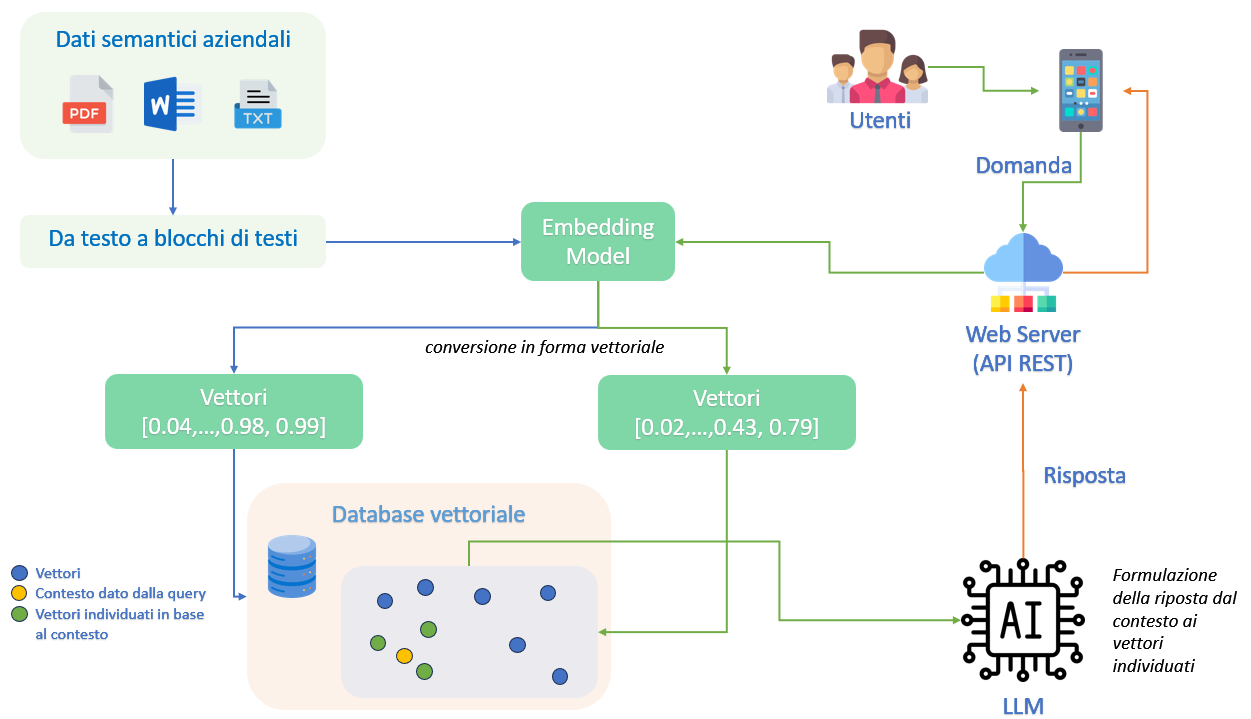
\includegraphics[width=0.8\textwidth]{img/architettura.png}
    \caption{Architettura del prodotto}
    \label{fig:architettura}
\end{figure}

\subsection{Funzionalità del prodotto}
Il prodotto avrà il compito di interagire con i propri utenti attraverso una webapp, rispondendo a domande su cataloghi di bevande. Ogni risposta sarà generata in linguaggio naturale, elaborando i dati tramite \textbf{BLOOM}. Le funzionalità principali includono:
\begin{itemize}
    \item \textbf{Interfaccia utente interattiva}: consente agli utenti di porre domande sul catalogo (\textit{es. descrizione di un prodotto o disponibilità in magazzino}) e di ricevere risposte immediate.
    \item \textbf{Motore di ricerca intelligente}: utilizza un sistema di embedding per trovare corrispondenze semantiche tra le domande degli utenti e i dati aziendali, estrae il contesto dai dati aziendali per fornire all'LLM dati accurati da elaborare.
    \item \textbf{Gestione dei dati}: accesso ai dettagli dei prodotti memorizzati in database relazionali, garantendo aggiornamenti in tempo reale. Costruzione di un database vettoriale per l'embedding delle parole.
    \item \textbf{Personalizzazione tramite backend}: gli amministratori possono configurare risposte predefinite(template di domanda e risposta), monitorare l’utilizzo e migliorare il sistema tramite feedback utente.
    \item \textbf{Apprendimento continuo}: il sistema evolve grazie ai feedback raccolti dagli utenti, migliorando la qualità delle risposte.
    \item \textbf{Compatibilità multi-dispositivo}: la piattaforma è progettata per essere accessibile 24/7 da mobile e desktop.
\end{itemize}

Il prodotto garantirà inoltre scalabilità e flessibilità, adattandosi a un’ampia gamma di aziende che desiderano offrire ai propri clienti un’esperienza di interazione avanzata e intuitiva.


\subsection{Tecnologie utilizzate} %TODO: Definire Tecnologie meglio
Possibili tecnologie da utilizzare per la realizzazione del prodotto:
\begin{itemize}
    \item \textbf{Embedding Model}: BERT, Sentence Transformers, OpenAI Embeddings.
    \item \textbf{Database Relazionale}: MySQL, PostgreSQL.
    \item \textbf{Database Vettoriale}: Pinecone, Weaviate, o FAISS.
    \item \textbf{LLM}: OpenAI GPT, BLOOM.
    \item \textbf{Web App}: React.
\end{itemize}

\subsection{Utenti finali}
Il prodotto è rivolto a aziende che desiderano offrire un servizio di assistenza 
clienti automatizzato e personalizzato. Gli utenti finali sono quindi i clienti 
delle aziende che interagiranno con l’assistente virtuale per ottenere 
informazioni sui prodotti e ricevere supporto.